%---------------------------------------------------------------------------------------------------
%		cpu.tex
%
%	This is file contains the cpu measurements.
%
%	Author: Andrea Meneghinello
% Version: 0.1
%	Table of changes:
%		21/03/2016 -> document definition
%---------------------------------------------------------------------------------------------------
\section{\acs{cpu} benchmark}
\label{sec:measurements-cpu}
By means of Linpack benchmark tool we want to measure the \acs{cpu} performance of both virtualization
environments. In order to have a basis for comparison we initially have executed the tool on the native
machine and then in various interesting environments, including:

\begin{enumerate}
	\item{one Docker container over the native \acs{os};}
	\item{one \ac{kvm} \ac{vm} with Hyper-Threading enabled;}
	\item{one \ac{kvm} \ac{vm} with Hyper-Threading disabled;}
	\item{one Docker container inside a \ac{kvm} \ac{vm} with Hyper-Threading enabled;}
	\item{one Docker container inside a \ac{kvm} \ac{vm} with Hyper-Threading disabled.}
\end{enumerate}

Even if running a container inside a \ac{vm} creates a double layer of virtualization, we also evaluated
these scenarios (2,3,4,5) because this is the only available solution if we choose a \ac{iaas} (like 
\ac{aws}) instead a \ac{paas} provider.

The \acs{cpu} tests were performed twice. The first time they where executed in complete isolation
in order to measure the overhead introduced by the virtualization layer; instead the second time they
were performed inserting an annoyance element that, casually, raised up and disturbed our computations.
This last one was performed to measure how the two virtualization types are able to adapt themselves
when they need to share the underlying hardware resources.

\subsection{Hyper-Threading Technology}
\label{sec:measurements-cpu-hyperThreadingTechnology}
Hyper-Threading (officially called Hyper-Threading Technology) is Intel's proprietary simultaneous
multi-threading implementation used to improve parallelization of computations performed on x86
microprocessors. Figure \ref{img:measurements-cpu-hyperThreading} shows an example of execution with
Hyper-Threading enabled.

\begin{figure}
	\centering{}
	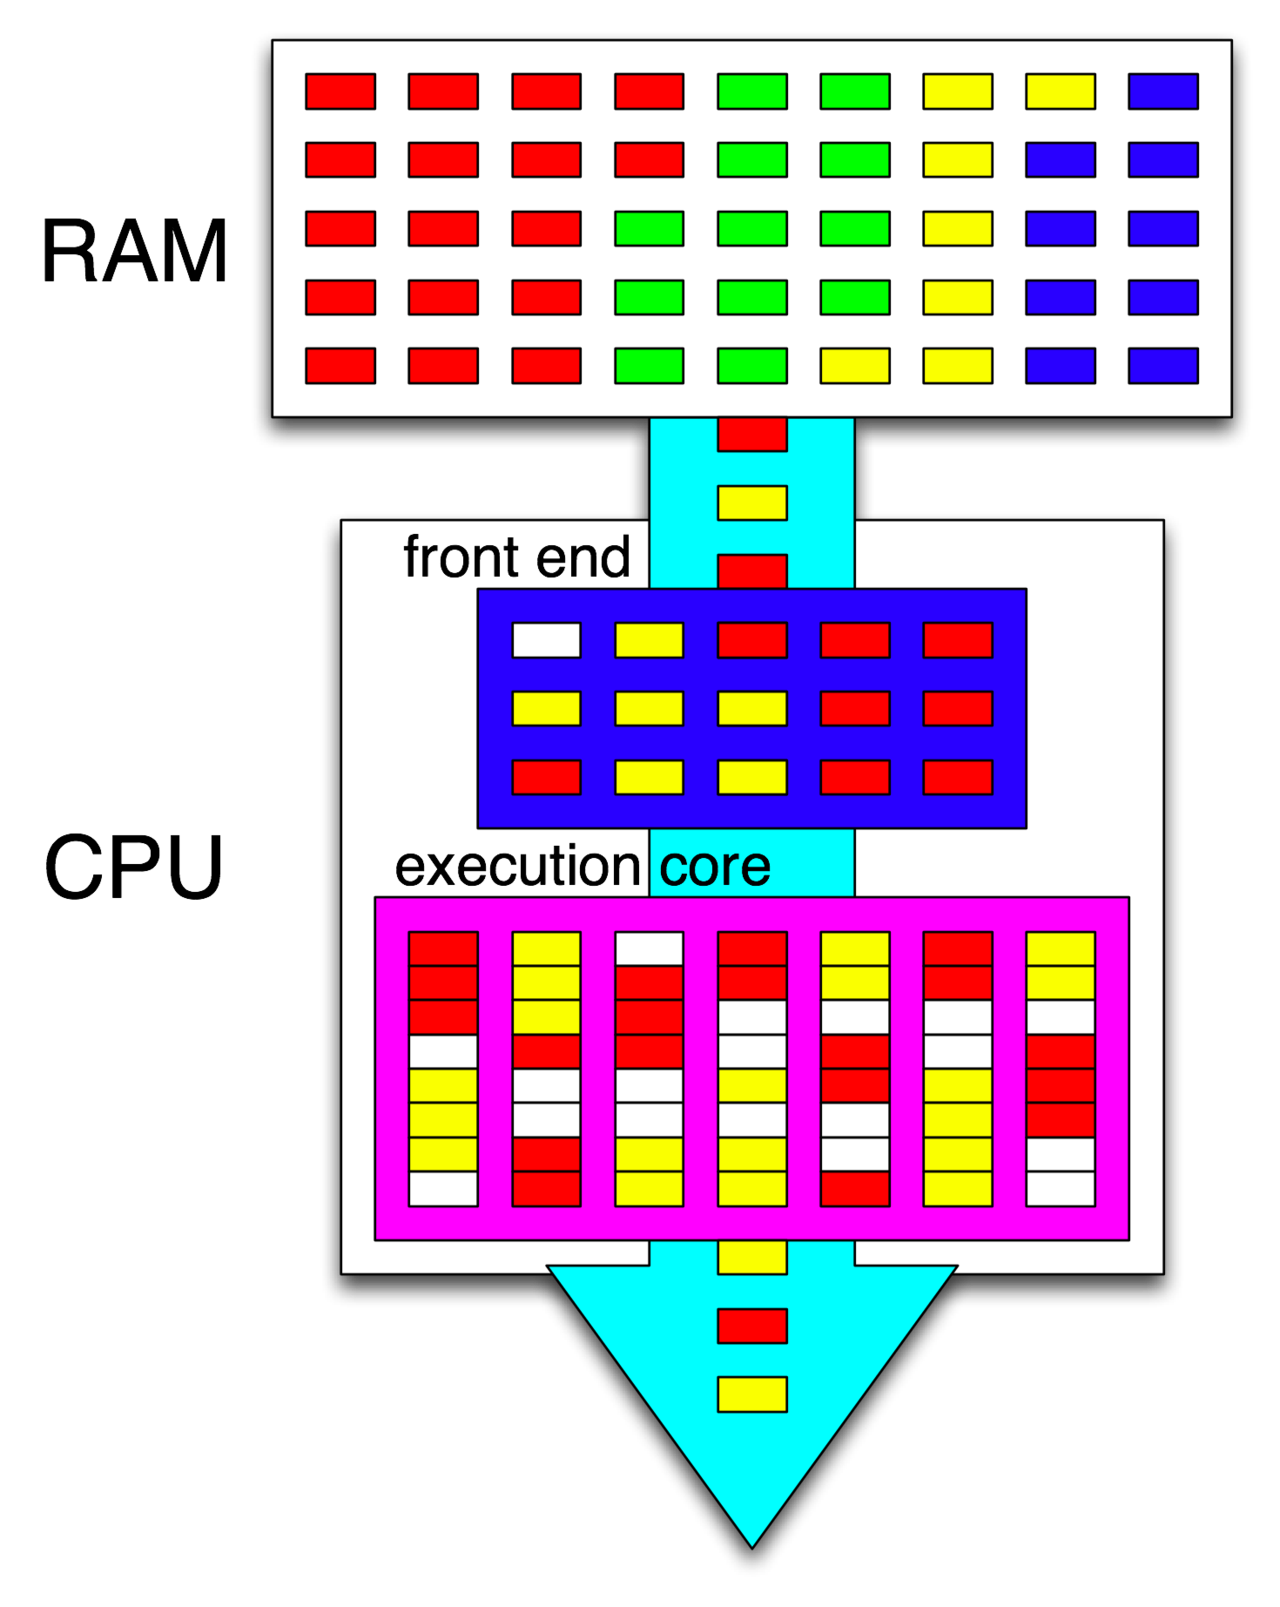
\includegraphics[width=0.35\textwidth]{chapters/measurements/images/hyper-threading.png}
	\caption[Overview of Intel Hyper-Threading]{A high-level depiction of the Intel's Hyper-Threading
		Technology: instructions are fetched from RAM (differently coloured boxes represent the instructions
		of four different programs), decoded and reordered by the front end (white boxes represent pipeline bubbles),
		and passed to the execution core capable of executing instructions from two different programs during
		the same clock cycle \cite{hyperthreading}.}
	\label{img:measurements-cpu-hyperThreading}
\end{figure}

For each processor core that is physically present, the \acs{os} addresses two virtual or logical cores,
and shares the workload between them when possible. The main function of Hyper-Threading is to increase
the number of independent instructions in the pipeline; it takes advantage of super-scalar architecture,
in which multiple instructions operate on separate data in parallel. With Hyper-Threading, one physical
core appears as two processors to the \acs{os}, allowing concurrent scheduling of two processes
per core. In addition, two or more processes can use the same resources: if resources for one process
are not available, then another process can continue if its resources are available.

In addition to requiring simultaneous multi-threading support in the \acs{os}, Hyper-Threading can be
properly utilized only with any \acs{os} specifically optimized for it. Furthermore, Intel recommends
to disable it when we are using an \acs{os} unaware of this hardware feature or in virtualized
environments.

\subsection{Linpack benchmark}
\label{sec:measurements-cpu-linpack}
\ac{hpl} \cite{linpackBenchmark} is a benchmark that measures the performance of a node or a cluster
using a workload that is characteristic of some scientific and technical applications. It is able to
solve a dense system of linear equations. Each system is represented as a matrix that will be divided
into smaller pieces, called ``tiles'', and distributed across the available processors or cluster's
nodes. Final performance is reported as the number of \ac{flops} achieved by the system. Users are able
to configure the benchmark varying the size of the problem and a number of parameters that describe
how the problem is solved. Some of the parameters describe how the problem is decomposed into tiles,
and how those tiles are distributed over the available resources.

The tool itself is a collection of subroutines that analyse and solve linear equations and linear
least-square problems. Originally was designed for supercomputers in the 1970s and early 1980s, it is able
to solves linear systems whose matrices are general, banded, symmetric indefinite, symmetric positive
definite, triangular, and triangular square. Linpack tool is built upon \ac{blas} package. It
uses LU factorization algorithm, similar to a technique commonly taught in college Linear Algebra courses,
called Gaussian elimination, but it is significantly improved to increase its numerical stability and
its performance.

Linpack library has largely been replaces by Lapack, which extends and improves upon the routines. In
Lapack, the routines have been carefully rewritten and tuned to take advantage of processors' cache,
available cores and relatively few references actually go to memory. In our tests, we used the
double-precision \ac{hpl} benchmark provided by Intel.

The benchmark produce a set of interesting values that describe the \ac{sut}, they are:

\begin{itemize}
	\item{\keyword{$R_{max}$}: which is the maximum measured performance in \ac{gflops};}
	\item{\keyword{$N$}: which represents the number of equations used to obtain $R_{max}$;}
	\item{\keyword{$R_{peak}$}: which represents the theoretical peak performance for the system; usually
		it is obtained by multiplying the number of processor cores, the processor frequency and the
		theoretical number of 64-bit vector floating-point results per clock;}
	\item{\keyword{$N_{1/2}$}: which represents the number of equations required to obtains one-half
		of the $R_{max}$ performance; it indicate the robustness of the system; a system with
		a small $N_{1/2}$ is able to operate well over a wide range of problems.}
\end{itemize}

With the preceding values we are also able to find the efficiency of the system through:

\begin{center}
	\begin{equation}
		efficienty = \frac{R_{max}}{R_{peak}}
	\end{equation}
\end{center}

Linpack \ac{hpl} is primarily a processor-core-intensive benchmark. It heavily exercises the vector
floating-point unit of each processor core. The faster the processor core and the more cores that are
available, the better are the benchmark performance. Data is moved from a memory into cache and used
heavily form cache, so larger caches do help. With current cache sizes of 1MB or more, most of
the current working data set already fits into cache, so memory performance is not seen as a major
factor in determining final performance. Instead a factor that affect the final performance is how
the tiles are defined and distributed.

The tool is used every year to compute the list of the major 500 super-computers in the world. After many
execution developers assert that good values are obtained finding a value for $N$ which saturate the
$80\%$ of the available main memory.

\subsection{Configuration}
\label{sec:measurements-cpu-configuration}
In order to respect the general convention (see in Section \ref{sec:measurements-cpu-linpack}) we found
a value for $N$ that is able to generate a system of linear-equations that saturate approximately the
$80\%$ of the available main memory; that is:

\begin{center}
	\begin{equation}
		N = \sqrt{\frac{available RAM * 1024^3}{8}}
	\end{equation}
\end{center}

that in our case correspond to $82\,897$ equations per system.

\subsection{Results}
\label{sec:measurements-cpu-results}
After executing the test in the environments described in Section \ref{sec:measurements-cpu} with the
configuration described in Section \ref{sec:measurements-cpu-configuration} we collected the execution
times (illustrated in Table \ref{tbl:measurements-cpu-results-time}) and the \acs{cpu}
capacity (illustrated in Table \ref{tbl:measurements-cpu-results-capacity}) for each listed
environment.

Actually the ``test number'' value, reported in the first column of each table, refers to test cases
of that list.

\begin{center}
	\begin{tabular}{| l | r | r | r | r | r |}
		\hline
		\multirow{2}{*}{Test num} &   \multicolumn{5}{c|}{\keyword{\acs{cpu} capacity without contention (\acs{gflops})}}   \\ \cline{2-6}
		                          & \textit{Min} & \textit{Max} & \textit{Avg} & \textit{Std. Dev.} & \textit{\% upon tot.} \\ \hline
		\textit{native}           & $286.3051$   & $303.0076$   & $293.1930$   & $6.3289$           & $100.000$             \\ \hline
		\textit{2}                & $266.4806$   & $306.6239$   & $285.4630$   & $12.8306$          & $97.364$              \\ \hline
		\textit{3}                & $84.3842$    & $86.4793$    & $85.9023$    & $0.7661$           & $29.299$              \\ \hline
		\textit{4}                & $94.1811$    & $95.3780$    & $95.0015$    & $0.4321$           & $32.402$              \\ \hline
		\textit{5}                & $84.2199$    & $88.0320$    & $85.9904$    & $1.3263$           & $29.329$              \\ \hline
		\textit{6}                & $91.5771$    & $94.2375$    & $93.1346$    & $0.8818$           & $31.766$              \\ \hline\hline
		\multirow{2}{*}{Test num} &    \multicolumn{5}{c|}{\keyword{\acs{cpu} capacity with contention (\acs{gflops})}}     \\ \cline{2-6}
		                          & \textit{Min} & \textit{Max} & \textit{Avg} & \textit{Std. Dev.} & \textit{\% upon tot.} \\ \hline
		\textit{native}           & $226.1955$   & $310.3253$   & $262.9988$   & $27.3098$          & $100.000$             \\ \hline
		\textit{2}                & $239.2409$   & $294.9315$   & $262.7408$   & $18.8278$          & $99.902$              \\ \hline
		\textit{3}                & $72.9531$    & $85.5957$    & $79.1688$    & $4.4305$           & $30.102$              \\ \hline
		\textit{4}                & $71.0966$    & $86.6270$    & $82.5354$    & $5.8239$           & $31.382$              \\ \hline
		\textit{5}                & $76.7307$    & $79.6143$    & $78.2996$    & $1.0309$           & $29.772$              \\ \hline
		\textit{6}                & $84.4720$    & $91.2945$    & $88.8362$    & $2.2995$           & $33.778$              \\ \hline
	\end{tabular}
	\captionof{table}{Resume of the \acs{cpu} capacity benchmark.}
	\label{tbl:measurements-cpu-results-capacity}
\end{center}

\begin{figure}
	\centering{}
	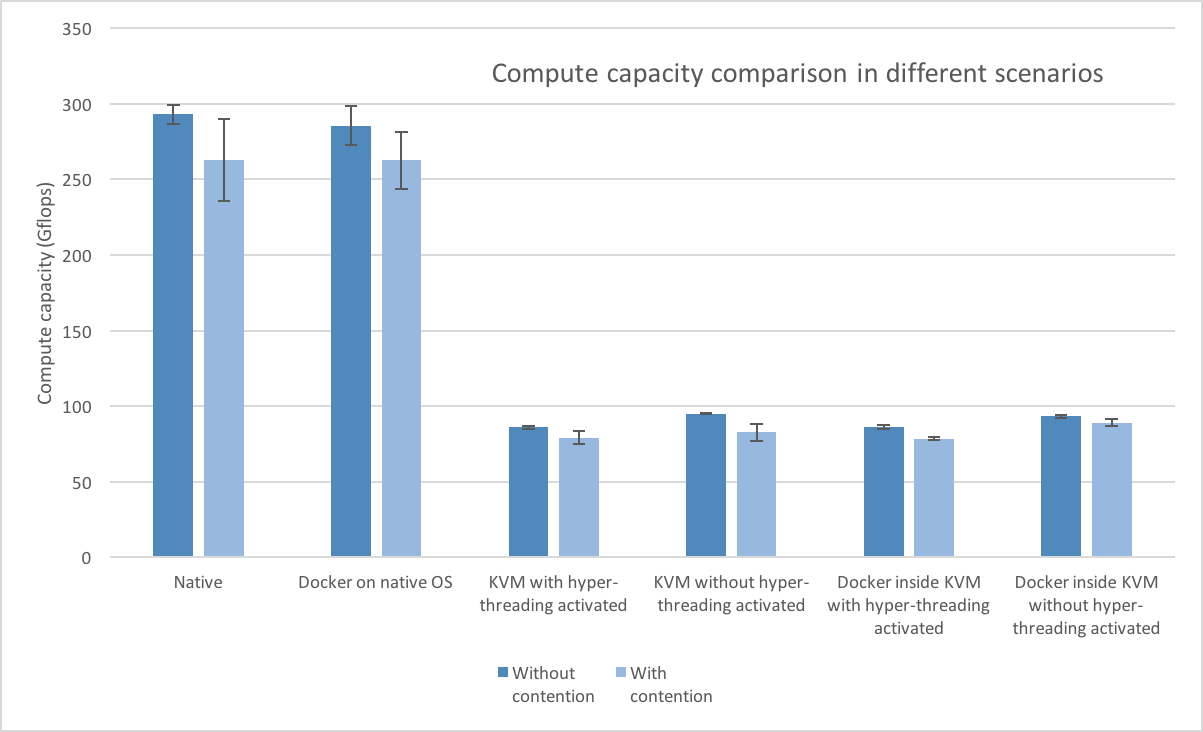
\includegraphics[width=0.75\textwidth]{chapters/measurements/images/cpu-capacity.png}
	\caption[Compute - resume of capacity benchmark]{Resume of \acs{cpu} capacity benchmark.}
	\label{img:measurements-cpu-results-capacity}
\end{figure}

In regard of \acs{cpu} capacity we can observe both from Table \ref{tbl:measurements-cpu-results-capacity}
and from chart \ref{img:measurements-cpu-results-capacity} that the \acs{os}-level virtualization,
provided by Docker, is able to exploit very well the \acs{cpu} capacity, both without and with contention.
The losses provided by that virtualization layer are approximatively from 1 to 3\%. Quite another thing is
the  hardware-level virtualization on which we collected losses approximatively from 68 to 71\% of the
\acs{cpu} compute capacity. This happens because the Linpack benchmark is highly adaptive and uses
system-provided information to tune itself to the architecture upon which it is running. The hardware-level
virtualization hides the totality of hardware information so the benchmark have to use generic algorithms
instead using optimizations.

In the matter of the double virtualization layer provided by inserting a Docker container inside a
\ac{kvm} \ac{vm} we do not find big differences from the execution without Docker inside the \ac{vm}.
In fact, we expect to find this results inasmuch Docker containers executing at the same level
of the \acs{os} on which they are based.

With respect to the capability of adapt themselves we have found better performance using
hardware-level virtualization instead the \acs{os}-level one, as the small standard deviation values
shows. We can affirm that this happens because the hardware-level virtualization is able to ``pin''
the underlying hardware resources to avoid over-scheduling.

Finally, as we expected executing relevant computation in virtualized environment that uses the Intel
Hyper-Threading Technology produces additional losses in \acs{cpu} capacity. Thus, the choice of
cloud provider of disable this feature produce a light increase of the performance.

\begin{center}
	\captionof{table}{Resume of \acs{cpu} capacity execution time.}
	\begin{tabular}{| l | r | r | r | r | r |}
		\hline
		\multirow{2}{*}{Test num} &               \multicolumn{5}{c|}{\keyword{Time without contention (s)}}                \\ \cline{2-6}
		                          & \textit{Min} & \textit{Max} & \textit{Avg} & \textit{Std. Dev.} & \textit{\% upon tot.} \\ \hline
		\textit{native}           & $1\,253.393$ & $1\,326.514$ & $1\,295.949$ & $27.747$           & $100.000$             \\ \hline
		\textit{2}                & $1\,238.611$ & $1\,425.198$ & $1\,333.098$ & $59.504$           & $102.867$             \\ \hline
		\textit{3}                & $4\,391.658$ & $4\,500.697$ & $4\,421.514$ & $39.941$           & $341.180$             \\ \hline
		\textit{4}                & $3\,981.921$ & $4\,032.526$ & $3\,997.138$ & $18.337$           & $308.433$             \\ \hline
		\textit{5}                & $4\,314.201$ & $4\,509.476$ & $4\,417.676$ & $67.989$           & $340.883$             \\ \hline
		\textit{6}                & $4\,039.111$ & $4\,147.189$ & $4\,080.002$ & $36.749$           & $314.827$             \\ \hline\hline
		\multirow{2}{*}{Test num} &                 \multicolumn{5}{c|}{\keyword{Time with contention (s)}}                 \\ \cline{2-6}
		                          & \textit{Min} & \textit{Max} & \textit{Avg} & \textit{Std. Dev.} & \textit{\% upon tot.} \\ \hline
		\textit{native}           & $1\,223.837$ & $1\,679.024$ & $1\,459.127$ & $146.186$          & $100.000$             \\ \hline
		\textit{2}                & $1\,287.715$ & $1\,587.470$ & $1\,452.694$ & $100.854$          & $99.559$              \\ \hline
		\textit{3}                & $4\,436.996$ & $5\,205.913$ & $4\,770.323$ & $259.307$          & $326.930$             \\ \hline
		\textit{4}                & $4\,384.173$ & $5\,341.855$ & $4\,773.795$ & $356.586$          & $327.168$             \\ \hline
		\textit{5}                & $4\,770.345$ & $4\,956.926$ & $4\,870.700$ & $75.448$           & $333.809$             \\ \hline
		\textit{6}                & $4\,254.526$ & $4\,698.309$ & $4\,396.572$ & $161.418$          & $301.315$             \\ \hline
	\end{tabular}
	\label{tbl:measurements-cpu-results-time}
\end{center}

\begin{figure}
	\centering{}
	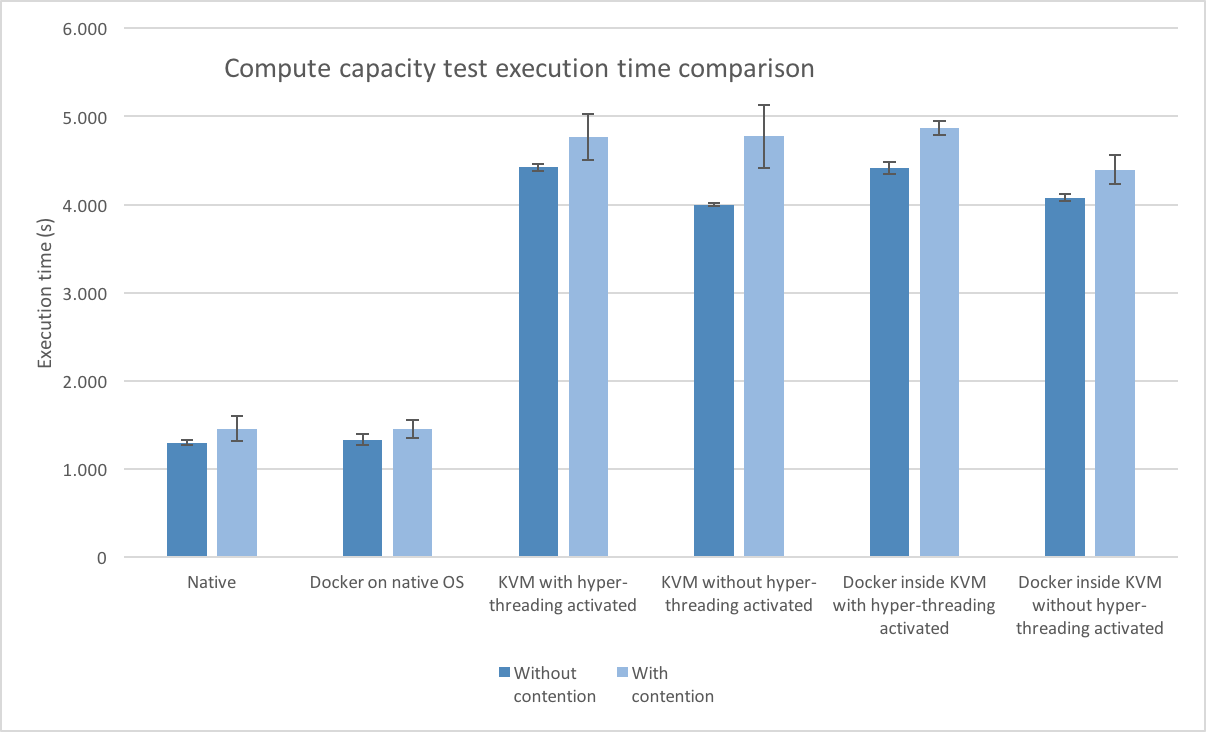
\includegraphics[width=0.75\textwidth]{chapters/measurements/images/cpu-time.png}
	\caption[Compute - resume of benchmark execution time]{Resume of benchmark execution time.}
	\label{img:measurements-cpu-results-time}
\end{figure}

As regards the execution time, we found that Docker containers are able to solve the problems
approximately in the same time as in the native execution, as Table \ref{tbl:measurements-cpu-results-time}
and chart \ref{img:measurements-cpu-results-time} shows. As we argued, this happens because
Docker containers execute at the same level of the \acs{os} on which they are based.

We have to pay specific attention to the presence or absence of Hyper-Threading Intel Technology. In fact,
keeping this feature enabled causes downgrade of the general performance.